\documentclass[a4paper]{article}
\usepackage{amsfonts}
\usepackage{amsmath}
\usepackage{amssymb}
\usepackage{graphicx}
\usepackage{float}

\begin{document}
  
\noindent \large Auteur: Siebe Mees \\
\noindent \large Studierichting: Informatica\\
\noindent \large Oefeningenreeks 5I nr. 2.2\\

\medskip

\normalsize

$f(x)=\ln(x^2-1) $ op $ \left[2,5\right]$\\
  
\begin{tabular}{c|ccc}

$x$ & $2$ & & $5$ \\ \hline

$f(x)$ & $\ln(3)$ & $+$ & $\ln(24)$ \\

$f'(x)$ &  & $+$ &  \\

$f''(x)$ &  & $-$ &  \\ \hline

$f(x)$ & $\ln(3)$ & $\nearrow$ & $\ln(24)$ \\

 &  & $\frown$ &  \\

\end{tabular}\\

\begin{figure}[H]
\centering
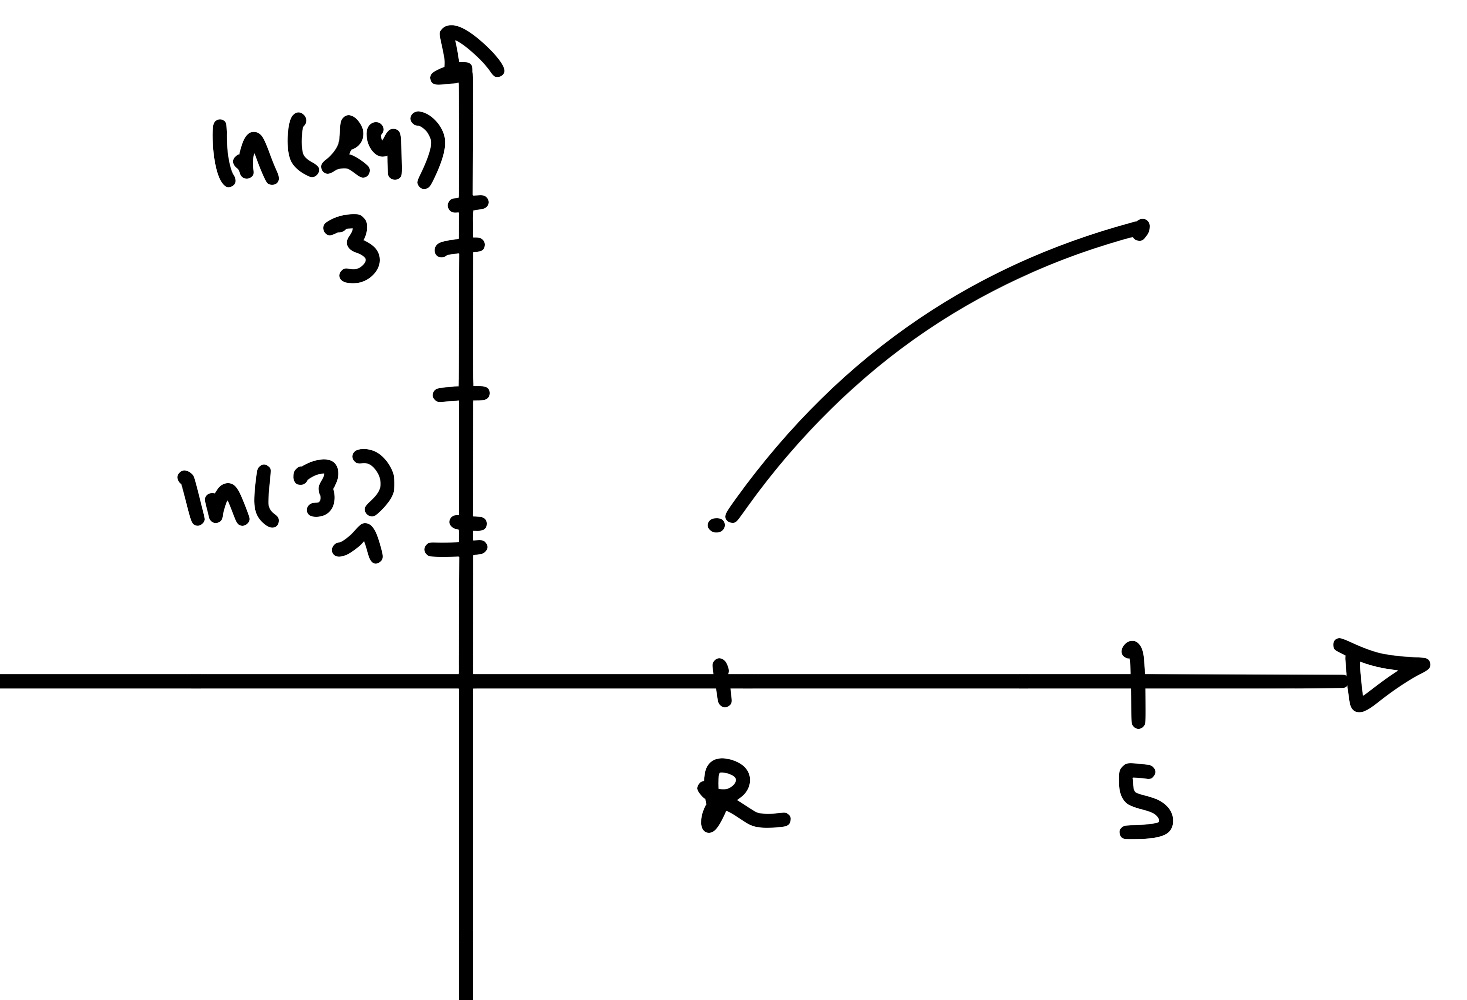
\includegraphics[width=5cm]{5I-2.2-siebe.mees.INF.png}
\end{figure}

$f'(x)=\dfrac{2x}{x^2-1}$\\

$L=\displaystyle\int_2^5 \sqrt{1+\left(f'(x)\right)^2} dx$\\

$=\displaystyle\int_2^5 \sqrt{1+\left(\dfrac{2x}{x^2-1}\right)^2} dx$\\

$=\displaystyle\int_2^5 \sqrt{1+\dfrac{4x^2}{(x^2-1)^2}} dx$\\

$=\displaystyle\int_2^5 \sqrt{\dfrac{(x^2-1)^2+4x^2}{(x^2-1)^2}} dx$\\

$=\displaystyle\int_2^5 \dfrac{\sqrt{x^4-2x^2+1+4x^2}}{x^2-1} dx$\\

$=\displaystyle\int_2^5 \dfrac{\sqrt{x^4+2x^2+1}}{x^2-1} dx$\\

$=\displaystyle\int_2^5 \dfrac{\sqrt{(x^2+1)^2}}{x^2-1} dx$\\

$=\displaystyle\int_2^5 \dfrac{x^2+1}{x^2-1} dx$\\

$=\displaystyle\int_2^5 \left(1+\dfrac{2}{x^2-1}\right) dx$\\

$=\displaystyle\int_2^5 \left(1+\dfrac{1}{x-1}-\dfrac{1}{x+1}\right) dx$\\

$=\left[x+\ln(x-1)-\ln(x+1)\right]_2^5$\\

$=\left(5+\ln 4-\ln 6\right)-\left(2+\ln 1-\ln 3\right)$\\

$=3+\ln\left(\dfrac{4}{6}\cdot\dfrac{3}{1}\right)$\\

$=3+\ln 2$\\

\begin{thebibliography}{999}
%\bibitem{a} Referentie
\end{thebibliography}
\end{document} 
